\section{Kết quả thực nghiệm và đánh giá giai đoạn 1}

Đúng với tính chất của Đồ án chuyên ngành (Giai đoạn 1), thay vì chỉ trình bày giao diện tĩnh, nhóm tập trung chạy các bộ thực nghiệm định lượng tự động trên hệ thống thực tế để kiểm chứng tính khả thi kỹ thuật của ba trụ cột cốt lõi: (i) sức mạnh và tốc độ phản hồi của hệ thống AI (tập trung vào quá trình xây dựng các thành phần nền tảng cho \textbf{Hybrid Bot} và kiểm định \textbf{LLM Bot}); (ii) hiệu quả băng thông và độ trễ của kiến trúc Multiplayer; và (iii) độ chính xác tái tạo khuôn mặt cùng tóc 3D của Smart Customization.

\subsection{Thực nghiệm đối kháng và đánh giá hệ thống AI}
Toàn bộ phép đo đối kháng AI được thực thi tự động ở chế độ mô phỏng không hiển thị đồ họa nhằm bảo đảm tốc độ và tính khách quan. Mỗi cặp đấu chạy từ $100$ đến $1{,}000$ ván đầy đủ, ghi nhận tự động tỷ lệ thắng, hòa, thua và thời gian suy nghĩ trung bình mỗi nước đi. Bảng \ref{tab:ai_benchmark_full} tổng hợp kết quả thực nghiệm qua các mốc tiến hóa thành phần tạo nên \textbf{Hybrid Bot} (từ học bắt chước, học tăng cường PPO đến kết hợp tìm kiếm Minimax và mạng đánh giá NNUE/Residual NNUE), kèm nhãn đối chiếu gọn trong ngoặc khớp với biểu đồ ở Hình \ref{fig:chart_ai_bench}.

\begin{table}[H]
    \centering
    \footnotesize
    \caption{Tổng hợp kết quả thực nghiệm đối kháng tự động giữa các mốc phát triển AI của Convergence Chess}
    \label{tab:ai_benchmark_full}
    \begin{tabularx}{\textwidth}{L{4.1cm} L{2.8cm} C{0.9cm} C{1.1cm} C{1.0cm} C{1.1cm} Y}
        \toprule
        \textbf{Mô hình thử nghiệm (P1)} & \textbf{Đối thủ chuẩn (P2)} & \textbf{Số trận} & \textbf{P1 thắng} & \textbf{Hòa} & \textbf{P2 thắng} & \textbf{Thời gian/nước (P1 vs P2)} \\
        \midrule
        Học bắt chước cơ sở (BC Template) & Minimax độ sâu 2 (Heu D2) & 100 & 1.00\% & 3.00\% & 96.00\% & -- \\
        Học bắt chước cải tiến (BC v2) & Minimax độ sâu 2 (Heu D2) & 100 & 12.00\% & 11.00\% & 77.00\% & -- \\
        Học bắt chước cải tiến (BC v2) & Minimax độ sâu 4 (Heu D4) & 100 & 18.00\% & 4.00\% & 78.00\% & -- \\
        Học tăng cường PPO tự đấu 27M bước (PPO Self-Play 27M) & Học bắt chước cơ sở (BC Template) & 100 & 87.00\% & 5.00\% & 8.00\% & -- \\
        Học tăng cường PPO tự đấu 27M bước (PPO Self-Play 27M) & Minimax độ sâu 2 (Heu D2) & 100 & 15.00\% & 6.00\% & 79.00\% & -- \\
        Học tăng cường có hàm giá trị (Critic Hybrid v4) & Minimax độ sâu 2 (Heu D2) & 1,000 & 23.90\% & 18.70\% & 57.40\% & 16 ms vs 11 ms \\
        Học tăng cường định hình thưởng (Heu RL v12p1) & Minimax độ sâu 2 (Heu D2) & 400 & 47.00\% & 26.25\% & 26.75\% & -- \\
        Học tăng cường thế hệ mới & Học tăng cường thế hệ trước & 500 & 44.80\% & 27.20\% & 28.00\% & 21 ms vs 21 ms \\
        Tìm kiếm lai mạng chính sách (NeuralMinimax) & Minimax độ sâu 2 (Heu D2) & 100 & \textbf{52.00\%} & 36.00\% & 12.00\% & 33 ms vs 6 ms \\
        Tìm kiếm lai mạng chính sách (NeuralMinimax) & Minimax độ sâu 3 (Heu D3) & 100 & \textbf{51.00\%} & 24.00\% & 25.00\% & 41 ms vs 10 ms \\
        Tìm kiếm lai mạng chính sách (NeuralMinimax) & Minimax độ sâu 4 (Heu D4) & 100 & 37.00\% & 30.00\% & 33.00\% & 38 ms vs 28 ms \\
        Mạng NNUE thế hệ 7, độ sâu 4 (NNUE Gen7) & Minimax độ sâu 4 (Heu D4) & 100 & 23.00\% & 49.00\% & 28.00\% & 238 ms vs 21 ms \\
        Hybrid Bot thế hệ 7 (NNUE + PPO) & Hybrid Bot thế hệ 3 & 100 & 33.00\% & 47.00\% & 20.00\% & 210 ms vs 218 ms \\
        \textbf{Mạng NNUE dạng dư thế hệ 7, độ sâu 4 (Residual NNUE Gen7)} & \textbf{Minimax độ sâu 4 (Heu D4)} & \textbf{100} & \textbf{51.00\%} & \textbf{28.00\%} & \textbf{21.00\%} & \textbf{66 ms vs 4 ms} \\
        Minimax độ sâu 1 (Heu D1) & Minimax độ sâu 6 (Heu D6) & 100 & 12.00\% & 10.00\% & 78.00\% & 6 ms vs 536 ms \\
        \bottomrule
    \end{tabularx}
\end{table}

\begin{figure}[H]
    \centering
    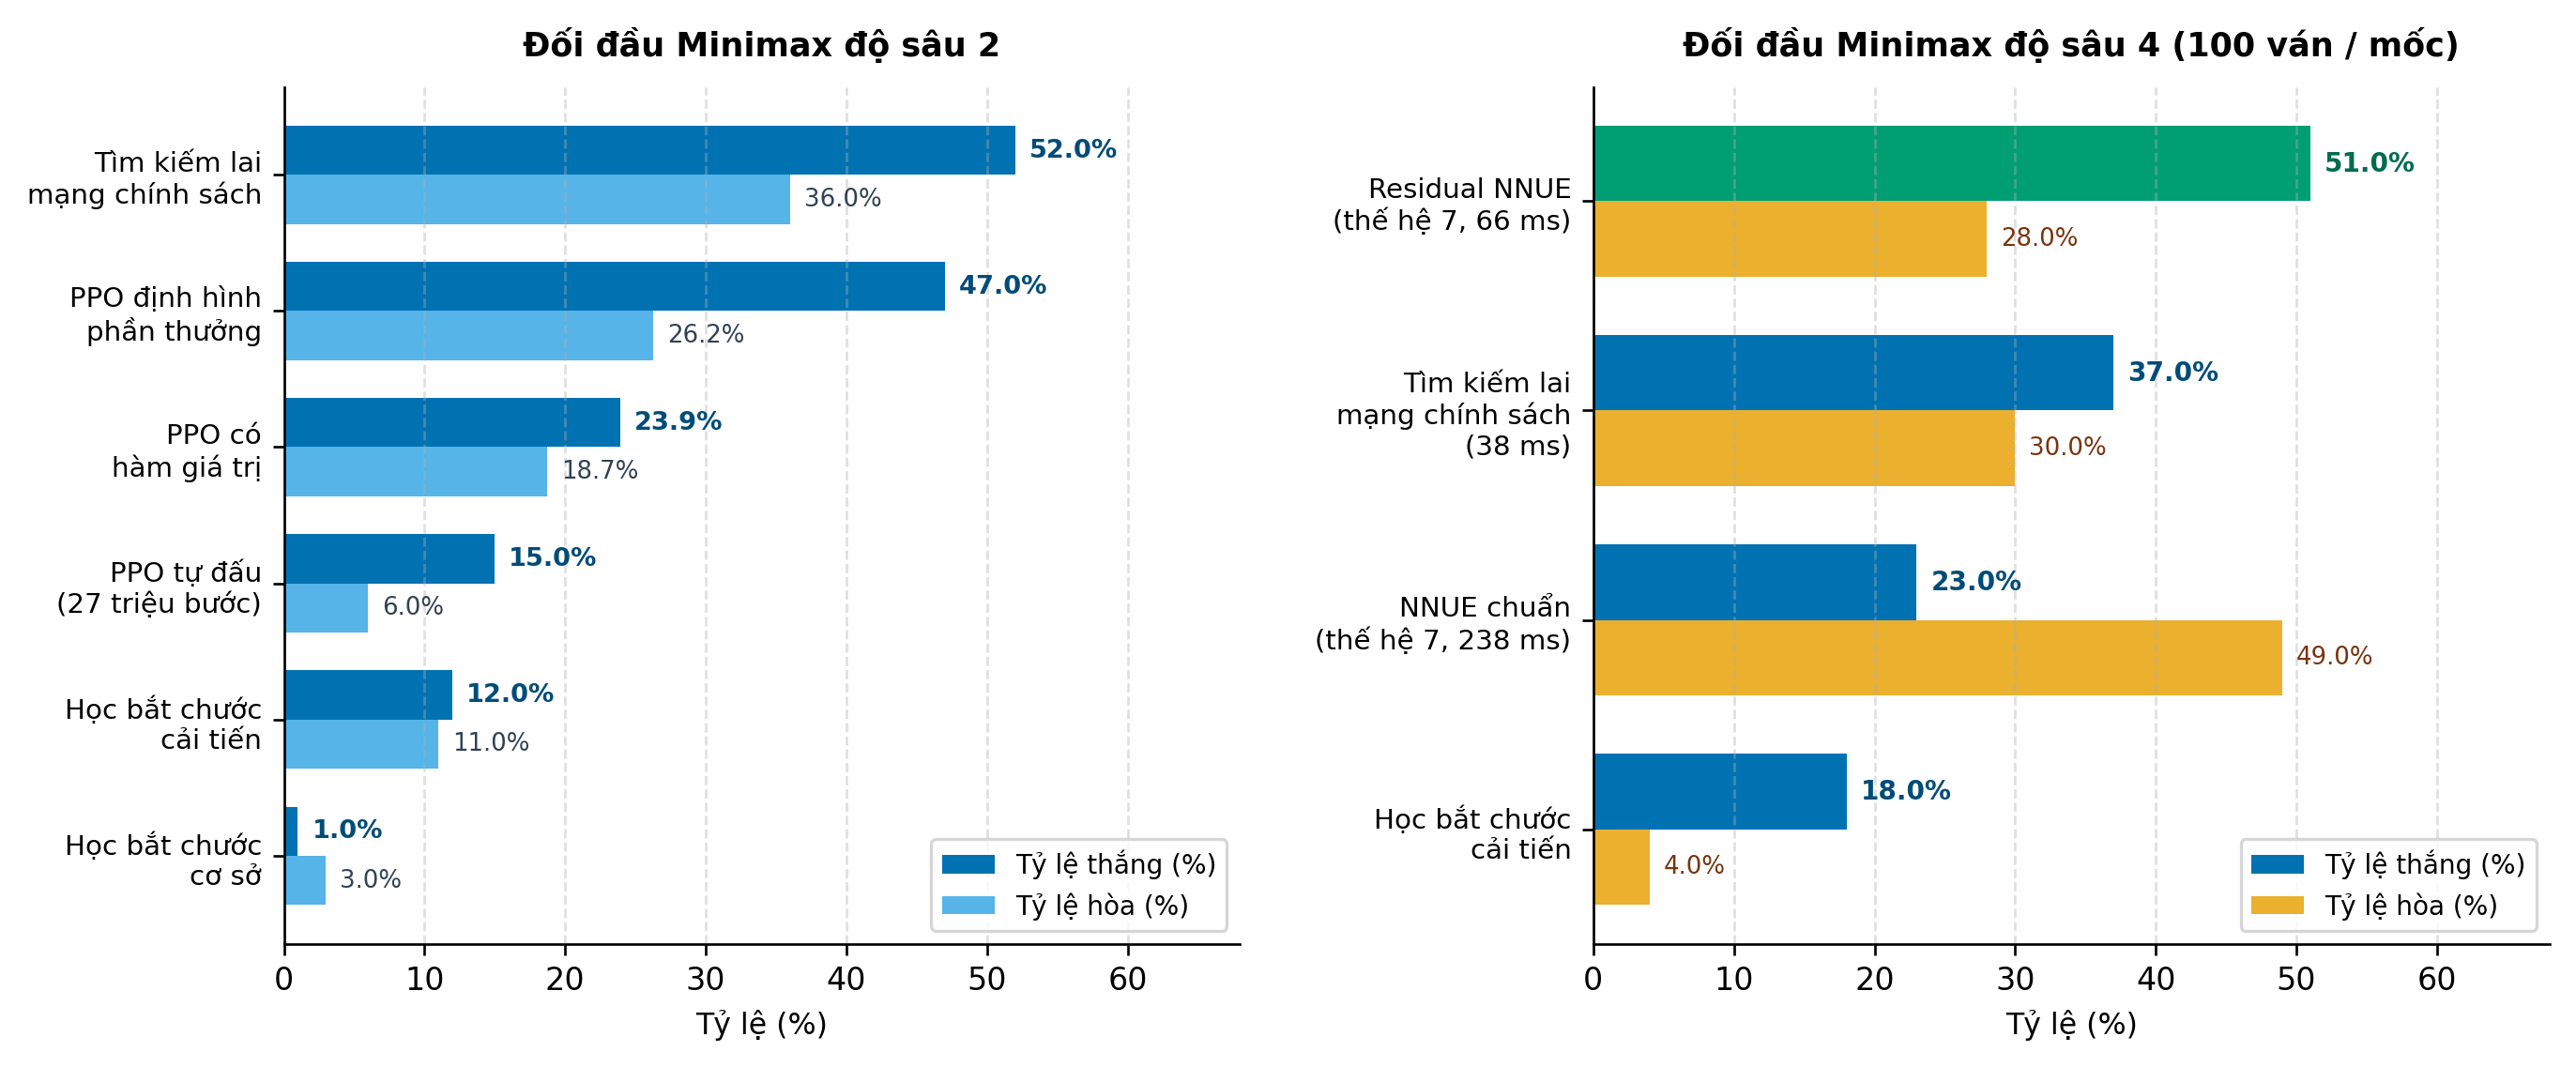
\includegraphics[width=\textwidth]{Diagrams/images/chart_ai_benchmark.png}
    \caption{Biểu đồ tiến triển tỷ lệ thắng của các mốc phát triển AI trước Minimax độ sâu 2 và độ sâu 4}
    \label{fig:chart_ai_bench}
\end{figure}

Từ Bảng \ref{tab:ai_benchmark_full} và Hình \ref{fig:chart_ai_bench}, nhóm rút ra bốn kết luận khoa học làm cơ sở định hình \textbf{Hybrid Bot} và \textbf{LLM Bot} sang Giai đoạn 2:
\begin{enumerate}
    \item \textbf{Giới hạn của mạng chính sách thuần túy không có tìm kiếm cây:} Dù mô hình học tăng cường PPO tự đấu áp đảo bản học bắt chước khởi tạo ($87.0\%$ so với $8.0\%$) và phản hồi rất nhanh (khoảng $16$--$21$ mili-giây mỗi nước), mạng chỉ nhìn một nước đi vẫn dễ mắc sai lầm chiến thuật ngắn hạn trước cây tìm kiếm Minimax do luật hợp thể và Surge tạo ra chuỗi ăn quân nhiều bước. Khi bổ sung định hình phần thưởng (Heu RL v12p1), tỷ lệ thắng trước Minimax độ sâu 2 tăng mạnh từ $15.0\%$ lên $47.0\%$ (vượt xa tỷ lệ thua $26.75\%$).
    \item \textbf{Hiệu quả rõ rệt của kiến trúc lai tìm kiếm và học sâu:} Khi dùng xác suất ưu tiên nước đi từ mạng chính sách dẫn đường cho cây tìm kiếm Minimax (NeuralMinimax), tác nhân áp đảo cả Minimax độ sâu 2 ($52\%$ thắng -- $12\%$ thua) lẫn độ sâu 3 ($51\%$ thắng -- $25\%$ thua) và nhỉnh hơn độ sâu 4 ($37\%$ -- $33\%$) chỉ với thời gian suy nghĩ $38$ mili-giây mỗi nước.
    \item \textbf{Bước đột phá của mạng đánh giá NNUE dạng dư trong Hybrid Bot:} So với mạng NNUE chuẩn cùng thế hệ dữ liệu thứ 7 ($23\%$ thắng, $238$ mili-giây mỗi nước), biến thể \textbf{NNUE dạng dư (Residual NNUE Gen7)} nâng tỷ lệ thắng trước Minimax độ sâu 4 lên tới \textbf{51.00\%} (chỉ thua $21.00\%$) đồng thời giảm thời gian suy nghĩ xuống còn \textbf{66 mili-giây mỗi nước} (nhanh hơn $3.6$ lần nhờ thứ tự đánh giá nút lá chính xác giúp cắt tỉa Alpha-Beta hiệu quả hơn).
    \item \textbf{Hiệu quả vòng lặp đồng huấn luyện đa thế hệ và kiểm định LLM Bot:} Phiên bản \textbf{Hybrid Bot thế hệ 7} đánh bại thế hệ 3 với tỷ số $33\%$ thắng -- $20\%$ thua ($47\%$ hòa), khẳng định hiệu quả của cơ chế tự sinh dữ liệu qua nhiều thế hệ. Song song đó, quy trình tiến hóa \textbf{LLM Bot} đã sàng lọc thành công $5$ mô-đun quy tắc chiến thuật vượt qua đủ $4$ cổng kiểm định tự động về tính an toàn, tốc độ, tính đối xứng và hiệu quả đối kháng cặp.
\end{enumerate}

\subsection{Đánh giá thực nghiệm hệ thống Multiplayer (Photon Fusion)}
Hình \ref{fig:chart_net_bench} trực quan hóa sự đánh đổi giữa băng thông và độ trễ từ phép đo 10 lần thăm dò trên Photon Fusion. Giao thức nhị phân tùy biến \texttt{OnlineDataBroadcastNetwork} trên kênh \texttt{Fusion Reliable Data} cắt giảm \textbf{78.1\%} tổng lưu lượng truyền tải (chỉ $70$ bytes so với $320$ bytes của \texttt{NetworkObject}) trong khi giữ tách biệt hoàn toàn với Core Domain. Các kịch bản kiểm thử đồng bộ giữa 2 máy khách và Khán giả (Spectator) đã xác nhận đồng bộ chính xác tên người chơi, danh sách slot, đội hình (\texttt{SquadData}), trạng thái sẵn sàng, hạt giống vật cản trung tuyến và luồng nước đi 4 bytes.

\begin{figure}[H]
    \centering
    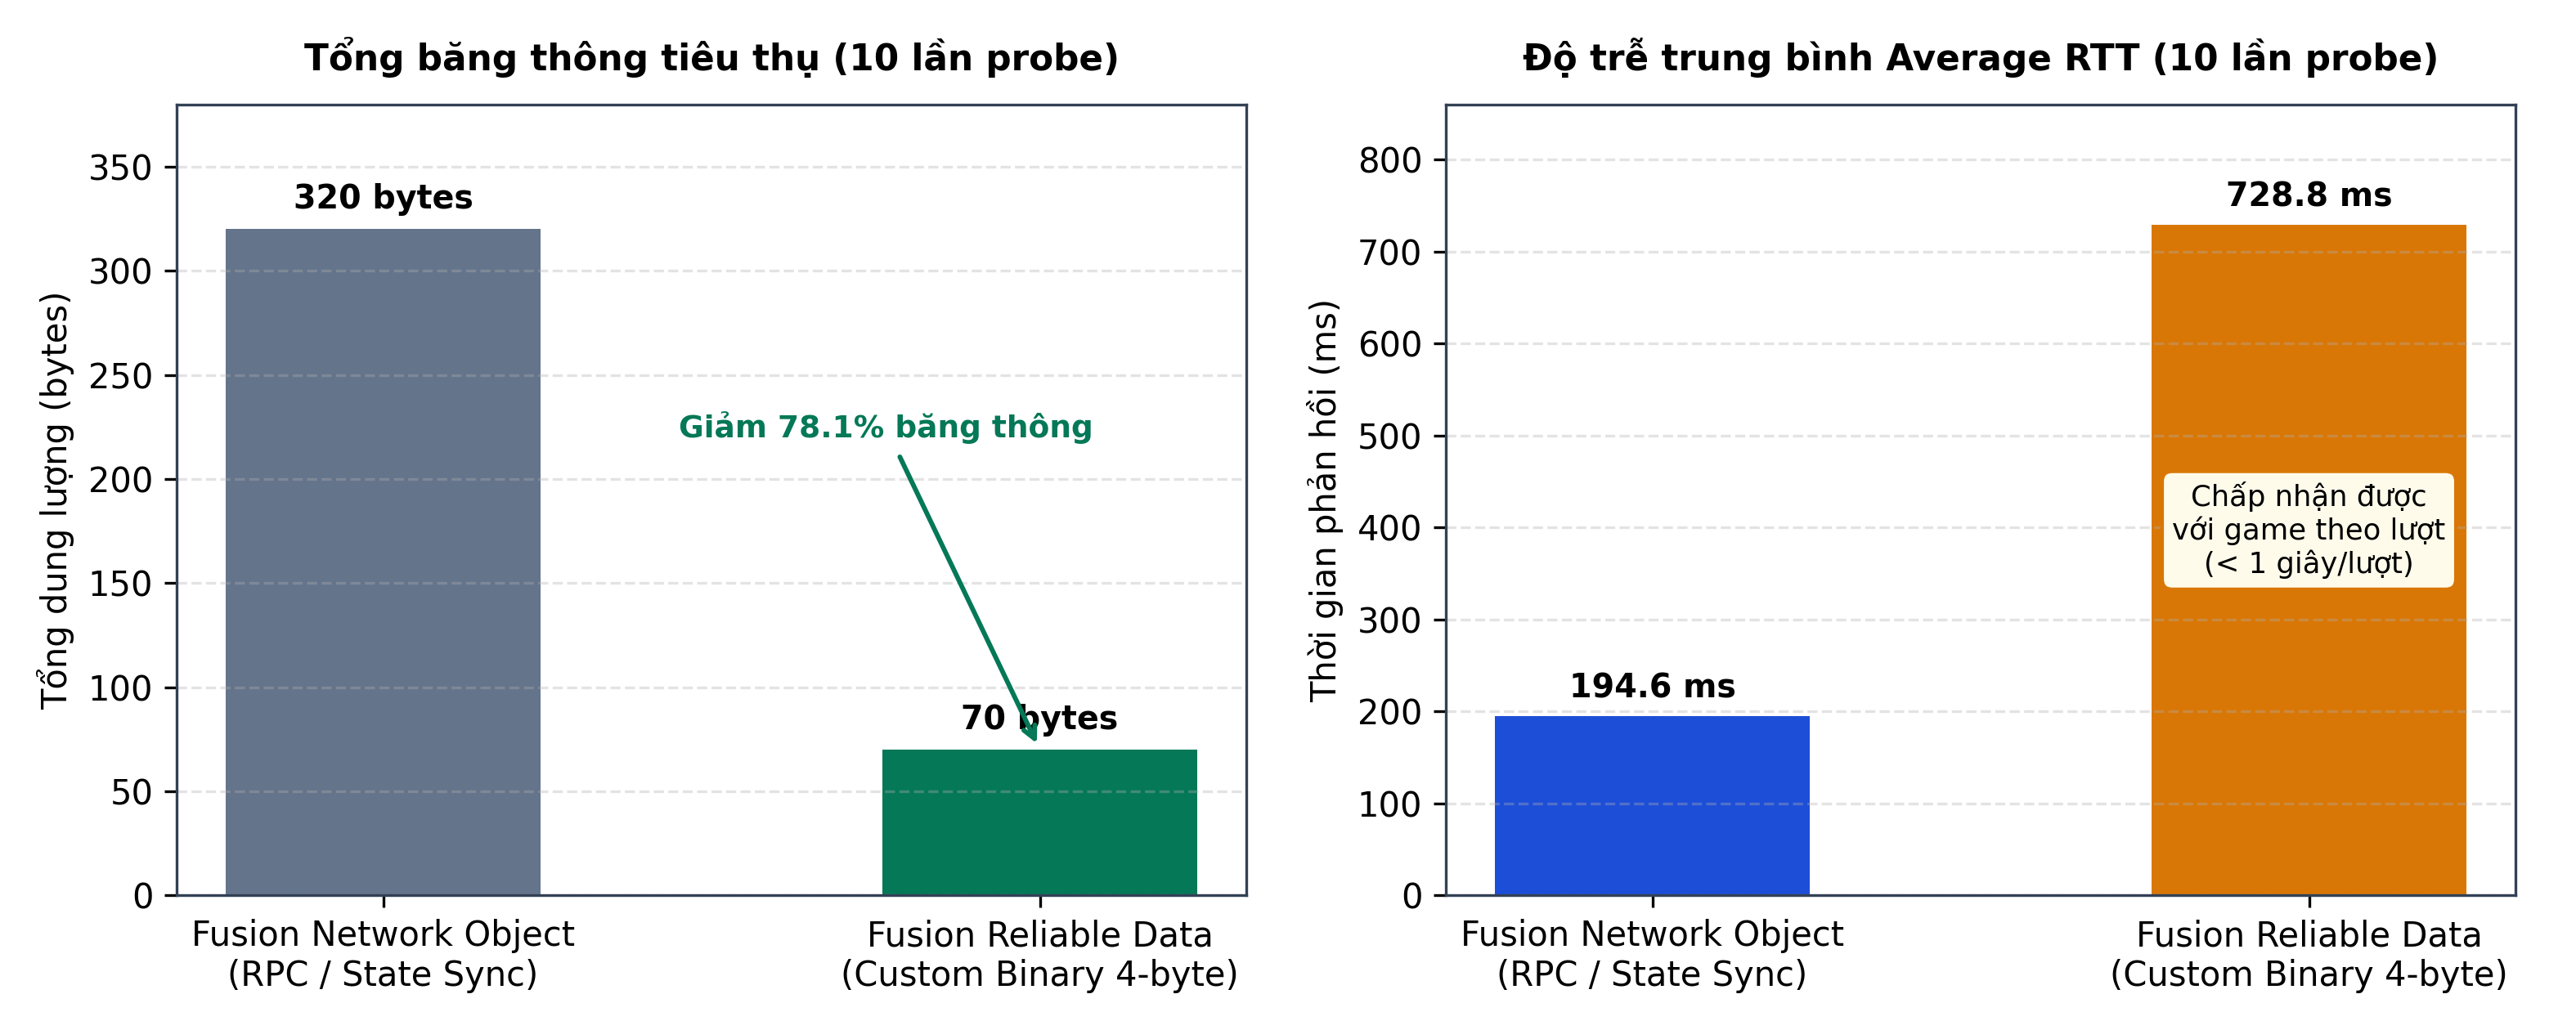
\includegraphics[width=0.95\textwidth]{Diagrams/images/chart_network_benchmark.png}
    \caption{So sánh định lượng băng thông tiêu thụ và Average RTT giữa hai cơ chế Photon Fusion}
    \label{fig:chart_net_bench}
\end{figure}

\subsection{Đánh giá thực nghiệm phân hệ tùy biến nhân vật 3D (Smart Customization)}
Trên máy trạm có cạc đồ họa NVIDIA GeForce RTX 4050 Laptop (bộ nhớ đồ họa 6 GB), quy trình tùy biến nhân vật 3D đã đạt được các kết quả kiểm chứng thực tế sau:
\begin{itemize}
    \item \textbf{Độ chính xác hình học khuôn mặt:} Sau khi tinh gọn về $25$ thông số hình thái độc lập và kiểm soát góc chụp khi sinh $24{,}000$ mẫu tổng hợp ($12{,}000$ Nam và $12{,}000$ Nữ), sai số tuyệt đối trung bình trên tập kiểm định sau $80$ chu kỳ huấn luyện giảm từ $0.0749$ ở phiên bản đầu xuống còn \textbf{0.0621} đối với mẫu Nam và \textbf{0.0616} đối với mẫu Nữ.
    \item \textbf{Chất lượng bề mặt da, khử bóng và thời gian xử lý:} Kết hợp chiếu ngược tam giác trên PyTorch3D kiểu MeInGame \cite{meingame}, khử bóng đối xứng hai bên trong không gian màu Lab, tách vùng hốc mắt, lọc bỏ vệt men răng và hòa trộn biên đa tầng (vùng chuyển tiếp $64$ điểm ảnh) giúp loại bỏ viền ghép gò má -- cổ và tránh hiện tượng bề mặt da bị bệt mờ như tượng sáp. Tổng thời gian xử lý toàn trình cho một ảnh chân dung ở chế độ tiêu chuẩn đạt khoảng \textbf{5.9 giây} trên máy tính cục bộ.
    \item \textbf{Hiệu quả hiển thị 3D trong Unity 6:} Hệ thống $6$ kiểu tóc 3D khớp chính xác vào da đầu, vật liệu mắt tạo đốm sáng tự nhiên trên giác mạc và bản đồ chi tiết nếp nhăn HRN có thể tinh chỉnh độ sâu trực tiếp trong trò chơi như minh họa tại Hình \ref{fig:sc_results}.
\end{itemize}

\begin{figure}[H]
    \centering
    \begin{subfigure}[b]{0.31\textwidth}
        \centering
        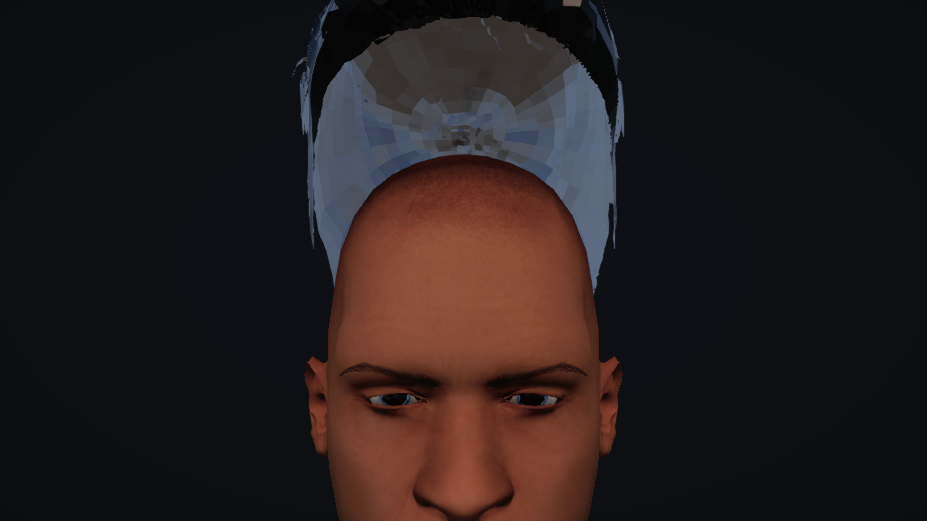
\includegraphics[width=\textwidth]{Content/Thực nghiệm và đánh giá/images/sc_hair_male_short01.png}
        \caption{Mẫu Nam kèm tóc ngắn kiểu 1}
    \end{subfigure}
    \hfill
    \begin{subfigure}[b]{0.31\textwidth}
        \centering
        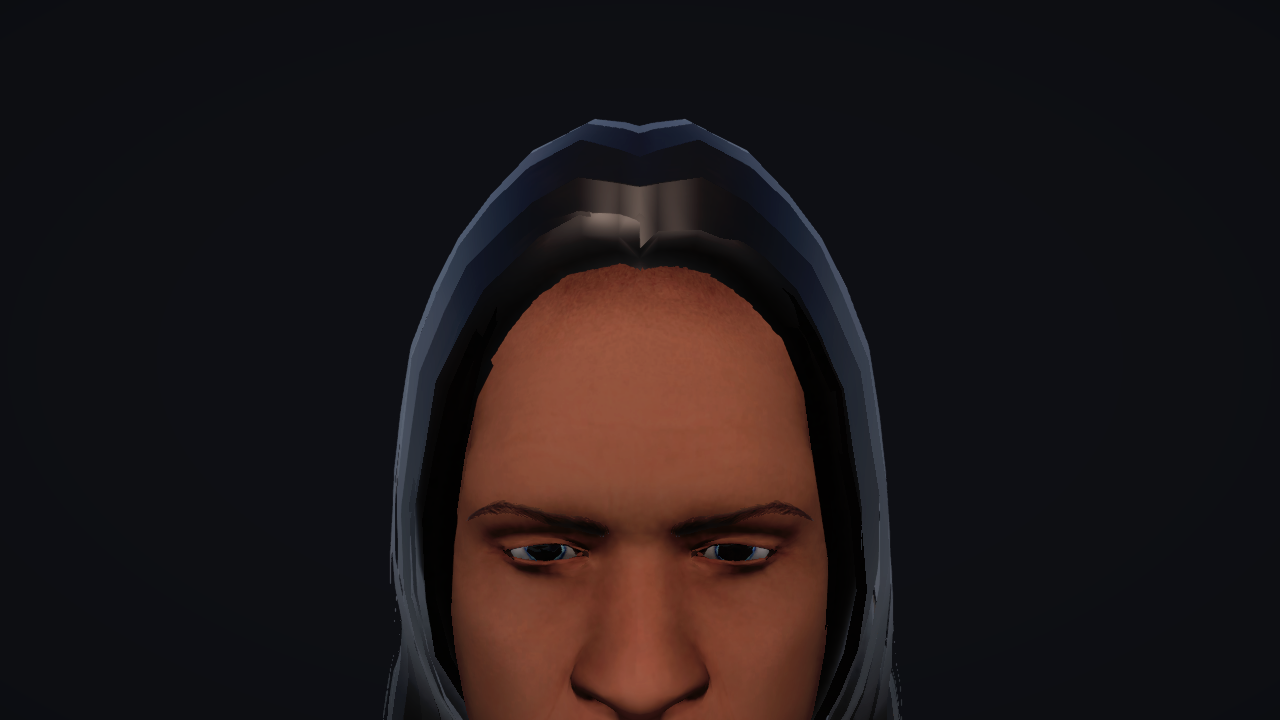
\includegraphics[width=\textwidth]{Content/Thực nghiệm và đánh giá/images/sc_hair_long01_verified.png}
        \caption{Mẫu Nữ kèm tóc dài}
    \end{subfigure}
    \hfill
    \begin{subfigure}[b]{0.31\textwidth}
        \centering
        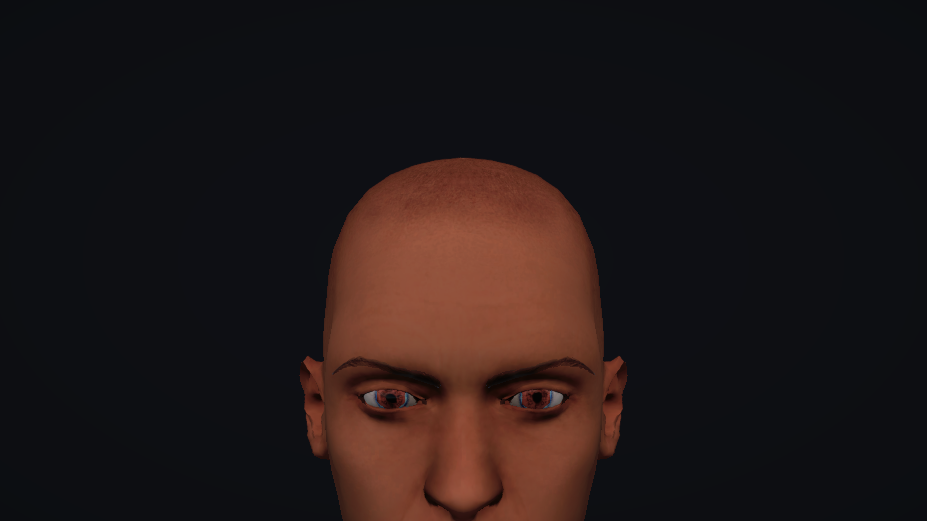
\includegraphics[width=\textwidth]{Content/Thực nghiệm và đánh giá/images/sc_hair_test_obama.png}
        \caption{Kiểm chứng tái tạo từ ảnh chân dung thực tế}
    \end{subfigure}
    \caption{Kết quả thực nghiệm tái tạo khuôn mặt, khử bóng da, vật liệu mắt và gắn tóc 3D trong Unity 6}
    \label{fig:sc_results}
\end{figure}

\begin{notebox}{Các hướng tiếp cận đã kiểm chứng loại bỏ hoặc tạm dừng trong giai đoạn 1}
Một giá trị thực nghiệm quan trọng của giai đoạn Đồ án chuyên ngành là sớm phát hiện và loại bỏ các phương án kém hiệu quả để tránh lãng phí nguồn lực ở Giai đoạn 2:
\begin{enumerate}
    \item \textbf{Dùng trực tiếp chiều sâu ước lượng từ MediaPipe:} Gây sai số trung bình bình phương tới $0.1415$ theo khoảng cách hai mắt (gấp $2.5$ lần sai số chiều ngang), buộc phải chuyển sang phương pháp sinh dữ liệu phối cảnh tổng hợp trực tiếp từ mô hình 3D gốc.
    \item \textbf{Huấn luyện mạng sinh kết cấu da trên dữ liệu tổng hợp:} Gây hiện tượng loang màu hồng nhân tạo quanh miệng và làm bề mặt da bệt mờ như tượng sáp; đã loại bỏ khỏi quy trình chính.
    \item \textbf{Khử bóng bằng mô hình khuếch tán IC-Light \cite{iclight}:} Dù khử bóng tốt (tốn khoảng $1.8$ giây riêng bước khuếch tán), mô hình này phụ thuộc bộ trọng số nặng và có nguy cơ làm thay đổi nét nhận dạng khuôn mặt gốc, do đó đã được tạm dừng để thay bằng chiếu ngược PyTorch3D kết hợp khử bóng đối xứng thuần giải phẫu.
    \item \textbf{Chuyển đổi trực tiếp bản đồ chi tiết bề mặt giữa hai chuẩn khuôn mặt khác nhau:} Gây đảo hướng ánh sáng tiếp tuyến do khác biệt góc xoay hệ tọa độ bề mặt; đã khắc phục bằng cách chuyển đổi bản đồ độ cao trước rồi mới tính lại độ dốc bề mặt trên hệ tọa độ của nhân vật đích.
    \item \textbf{Gắn trực tiếp mô hình tóc rời bằng khung xương mặc định hoặc dịch tọa độ thủ công:} Gây lệch tư thế gốc khiến tóc bị rơi xuống thấp hoặc chìm $4$--$5$ cm vào trong hộp sọ; đã chuẩn hóa hoàn toàn bằng công cụ định vị da đầu của MPFB v2.
\end{enumerate}
\end{notebox}

\subsection{Kết quả giao diện nguyên mẫu các màn hình trò chơi}
Bên cạnh các kết quả định lượng về AI, mạng và Smart Customization, nguyên mẫu chơi thử đã kết nối hoàn chỉnh các màn hình điều hướng chính trong Unity 6. Ba khung hình dưới đây đánh dấu các góc chụp giao diện thực tế từ bản dựng hiện tại để nhóm bổ sung ảnh chụp màn hình trước khi in nộp:

\begin{figure}[H]
    \centering
    \screenshotplaceholder{Content/Thực nghiệm và đánh giá/images/ui\_mainmenu\_squad.png}{Chụp ảnh màn hình chính và giao diện xây dựng đội hình đang kéo thả quân cờ trong ngân sách 12 điểm.}
    \caption{Giao diện màn hình chính và màn hình thiết lập đội hình}
    \label{fig:ui_squad_placeholder}
\end{figure}

\begin{figure}[H]
    \centering
    \screenshotplaceholder{Content/Thực nghiệm và đánh giá/images/ui\_lobby\_online.png}{Chụp ảnh màn hình sảnh chờ PvP Online (UIPopupLobby) thể hiện lựa chọn Photon Region, mã phòng, 3 nhóm vị trí (Trắng, Đen, Khán giả) và trạng thái Sẵn sàng.}
    \caption{Giao diện sảnh chờ PvP Online hỗ trợ phân vai và đồng bộ đội hình}
    \label{fig:ui_lobby_placeholder}
\end{figure}

\begin{figure}[H]
    \centering
    \screenshotplaceholder{Content/Thực nghiệm và đánh giá/images/ui\_ingame\_6x6.png}{Chụp ảnh trận đấu thực tế trên bàn cờ 3D 6x6 gồm bộ quân cờ Trung cổ, ô vật cản trung tuyến, vùng tô sáng nước đi/hợp thể và bảng thông số trong trận.}
    \caption{Giao diện bàn cờ 3D 6x6 và bảng thông số chiến thuật trong trận đấu}
    \label{fig:ui_ingame_placeholder}
\end{figure}
